\documentclass[twocolumn,10pt]{asme2ej}
\usepackage{epsfig}
\usepackage{graphicx}
\graphicspath{ {./figure/} }

\title{NAOlution: Using Convolutional neural network to navigate robot NAO towards an object}

\author{Martin Kostelansky
    \affiliation{
	Faculty of Informaion Technology\\
	Czech Technical University\\
	Prague, Czechia\\
    Email: kostema3@fit.cvut.cz
    }	
}

\begin{document}

\maketitle
\begin{abstract}
{\it NAOlution has researched training Convolutional neural network to \
navigate robot NAO towards an object using an image input. Convolutional \
Neural networks have been trained by genetic algorithm in the real-time \
simulation. Nets have been trained by this method to navigate robot NAO \
towards "plant like object" in simulation.}

\end{abstract}

\section{Introduction}
Convloutional neural networks have been widely used for many purposes \
such as classification or localization. In our research we have tried to \
use lightened CNNs to navigate robot NAO in real-time simulation towards \
an object. The architecture of the network was inspired by VGG\cite{VGG16}. To \
train such networks we used genetic algorithm. Which were ranked \ 
by the distance of the robot from the target. By this method we were \
able to train a model to come to close distance of the selected object.

\section{Network architecture}
\label{sec:architecture}
The network's architecture was mainly inspired by deep convloutional \
neural nets used for image recognition such as VGG\cite{VGG16}. The \
architecture was lightened down to use this network for multiple \
frames per second.
\subsection{Input}
The imagees from NAO's camera were resized to $128x128$ pixels \
grayscale, so the input dimension was $128x128x1$, where were \
the values from interval $(0,255)$.
\subsection{Convolutional and pooling layers}
The first layer was a maxpooling layer with receptor field $2x2$ \
pixels and the spatial resolution of the output from this layer \
is thus $64x64x1$. This layer follow two convolutional layers \
both with four feature maps with receptor field $4x4$ pixels \
and bias equals to one. The next sequence of convolutional layers \
is separated by maxpooling pooling layer with receptor field \
$4x4$ pixels. Second block of convolutional block is composed \
from two layers, both with eight feature maps and receptor fields \
$4x4$ pixels. Last layer is again maxpooling layer with receptor \
field $2x2$ pixels.
\par Every convolutional layer was initialized to random value from\
normal distribution with mean $0.0$ and standard deviation \
$0.05$.

\subsection{Fully connected layers}
Convolutional and pooling layers are followed by two fully connected \
layers, both of them contains eight neurons activated by \textsc{ReLu} \
function and their weights were randomly selected from normal \
distribution with mean $0.0$ and standard deviation $0.05$.

\subsection{Output layer}
Output layer has only three neurons, all of them use as an activation \
function \textsc{TanH} function and were randomly selected from normal \
distribution with mean $0.0$ and standard deviation $0.05$.\
\par Every output from these layers features robot's velocity \
towards/backward, left/right and left/right spin.

\begin{figure}[ht]
\begin{center}
    \begin{tabular}{ |c|c| } 
     \hline
     Layer & Dimension \\ 
     \hline
     \hline  
     Input & 128x128x1 \\ 
     \hline
     MaxPool1 & 2x2, stride 1 \\ 
     \hline
     Conv1 & 4x4, 4 x 2 \\
     \hline
     MaxPool2 & 2x2, stride 1 \\ 
     \hline
     Conv2 & 4x4, 4 x 2 \\ 
     \hline
     MaxPool3 & 2x2, stride 1 \\
     \hline
     FC1 & 16 relu \\
     \hline
     FC2 & 16 relu \\
     \hline
     FC3 & 3 tanh \\
     \hline
    \end{tabular}
    \end{center}
    \caption{Distance from the target during the evolution.}
    \label{fig:tbl}
\end{figure}

\section{Evolution algorithm}
During the evolution was created a population containing $50$ individuals \
created by process described in section~\ref{sec:architecture}. Each individual was evaluated \
by the distance from the target. Individual simulation run lasted until \
the robot comes to a target or until the timeout. After each epoch \
was created a new generation by crossing layers of two individuals. \
Individuals for crossing were randomly selected from normal distribution \
with mean $0.0$ and standard deviation equals to $30\%$ of the population \
size. Evolution ran for $30$ generations. The figure~\ref{fig:gr} describes \
average, best and worst performance.

\begin{figure}[ht]
    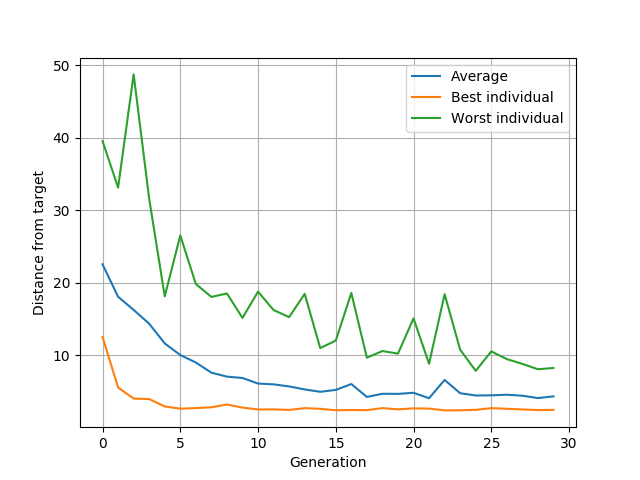
\includegraphics[width=0.45\textwidth]{evolution.png}
    \caption{Distance from the target during the evolution.}
    \label{fig:gr}
\end{figure}

\section{Conclusion}
In this work we have shown that it's possible to use Convolutional neural \
networks to navigate robot towards an object in real time simulation. \
To use train CNN to navigate the robot NAO towards an object in multiple \
positions, or to generalize the target object would be needed more simulations \
with different positions and different "similar objects" (e.g. in our case \
different "plant like objects"). Based on the research when was trained robotic \
arm to manipulate cubes \cite{OAI} to highlight the target object would be also \
needed to change background and floor to multiple patterns during the training.

\begin{acknowledgment}
I'd like to thank Faculty of Information Technology CTU in Prague for the \
opportunity and resources to make this reasearch happened. I'd also like to thank to \
professor Pablo Maldonado for many consultations and valuable advises during \
my work.
\end{acknowledgment}

\bibliographystyle{asmems4}
\bibliography{asme2e}

\end{document}